\begin{flushleft}
{\color{Blue}{\subsection{Mock-ups}}}

For what concern the software-to-be mockups, is possible to find them in \textit{Section 3.1} in the \textit{Requirements Analysis and Specification Document}.\\
As for reminder for the next section, for the Data4Help part, the user section is intended to be a mobile application and the Third Party section a website. On the other hand for AutomatedSOS part the idea is to have only a mobile application.
{\color{Blue}{\subsection{UX Diagrams}}}

The following diagrams are intended to give a general idea about the interactions between the various screens and the actions that are permitted.
For the sake of clarity here are explained the notation of the interfaces:
\begin{itemize}
\item \textbf{\textit{<<Screen>>:}} the screen is what the final user is going to see.
\item \textbf{\textit{<<Input Form>>:}} everything that the final user is going to interact with (empty space to fill with text, checkboxes, on/off buttons...).
\item \textbf{\textit{<<Screen Compartment>>:}} part of the screen that contains plain text.
\end{itemize}

{\color{Blue}{\subsubsection{Data4Help}}}

\textbf{User}

\begin{figure}[H]
	\centering
	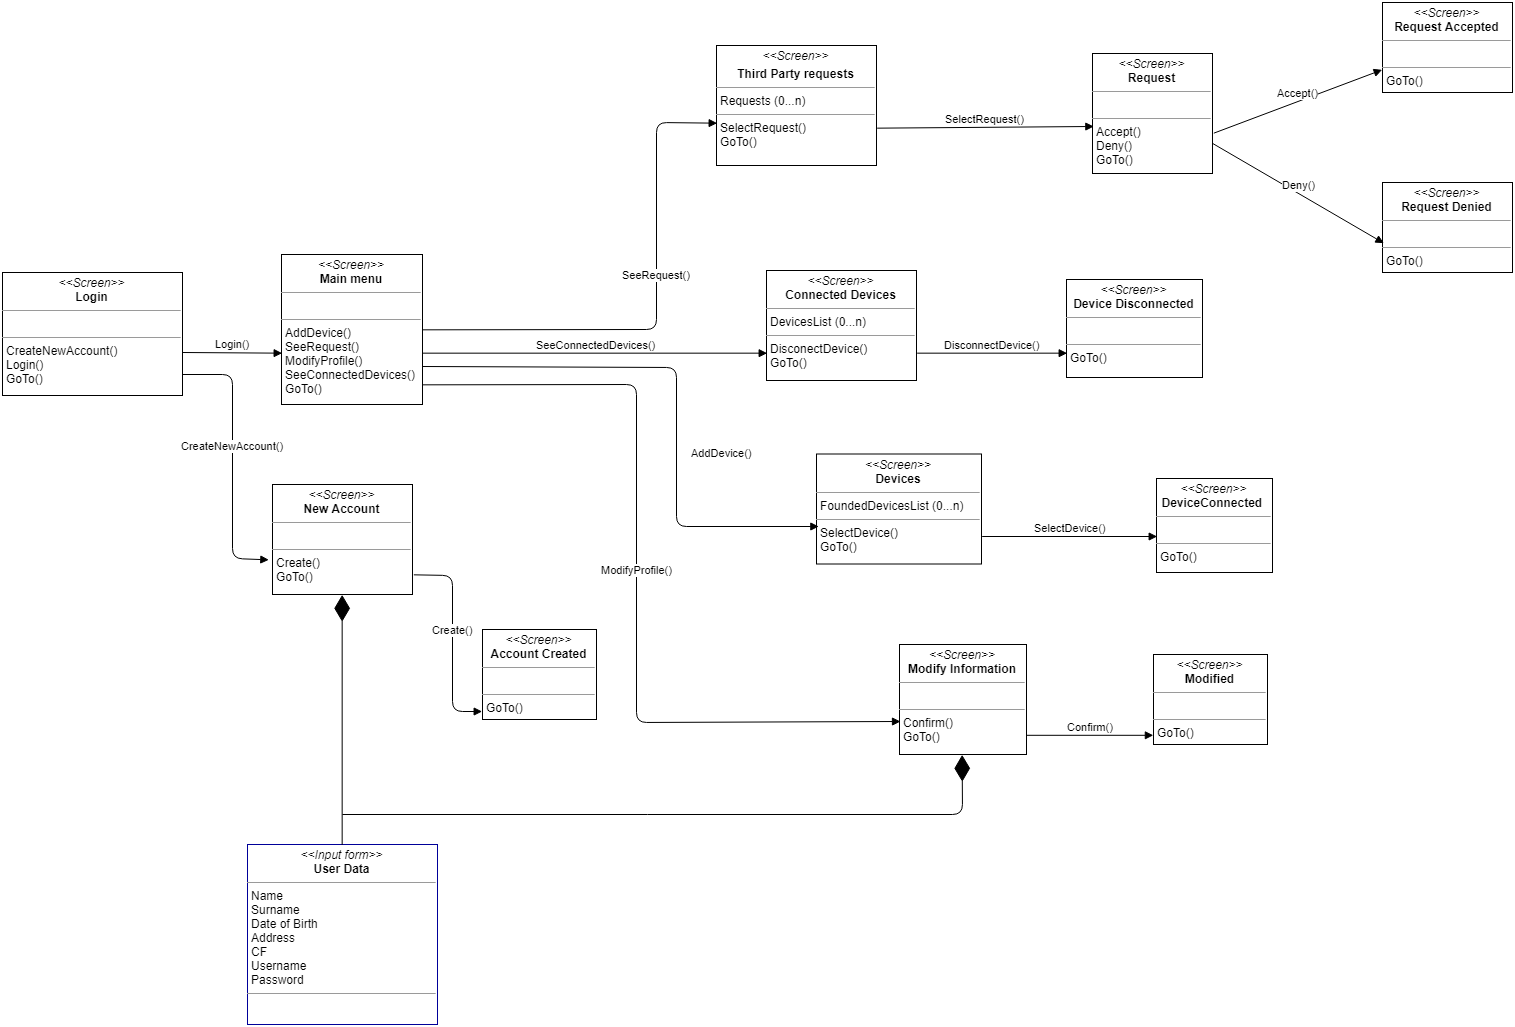
\includegraphics[scale=0.3]{Images/User_interface/Trackme-Data4Helpuser}
	\caption{Data4Help User UX diagram}
\end{figure}
\newpage
\textbf{Third Party}

\begin{figure}[H]
	\centering
	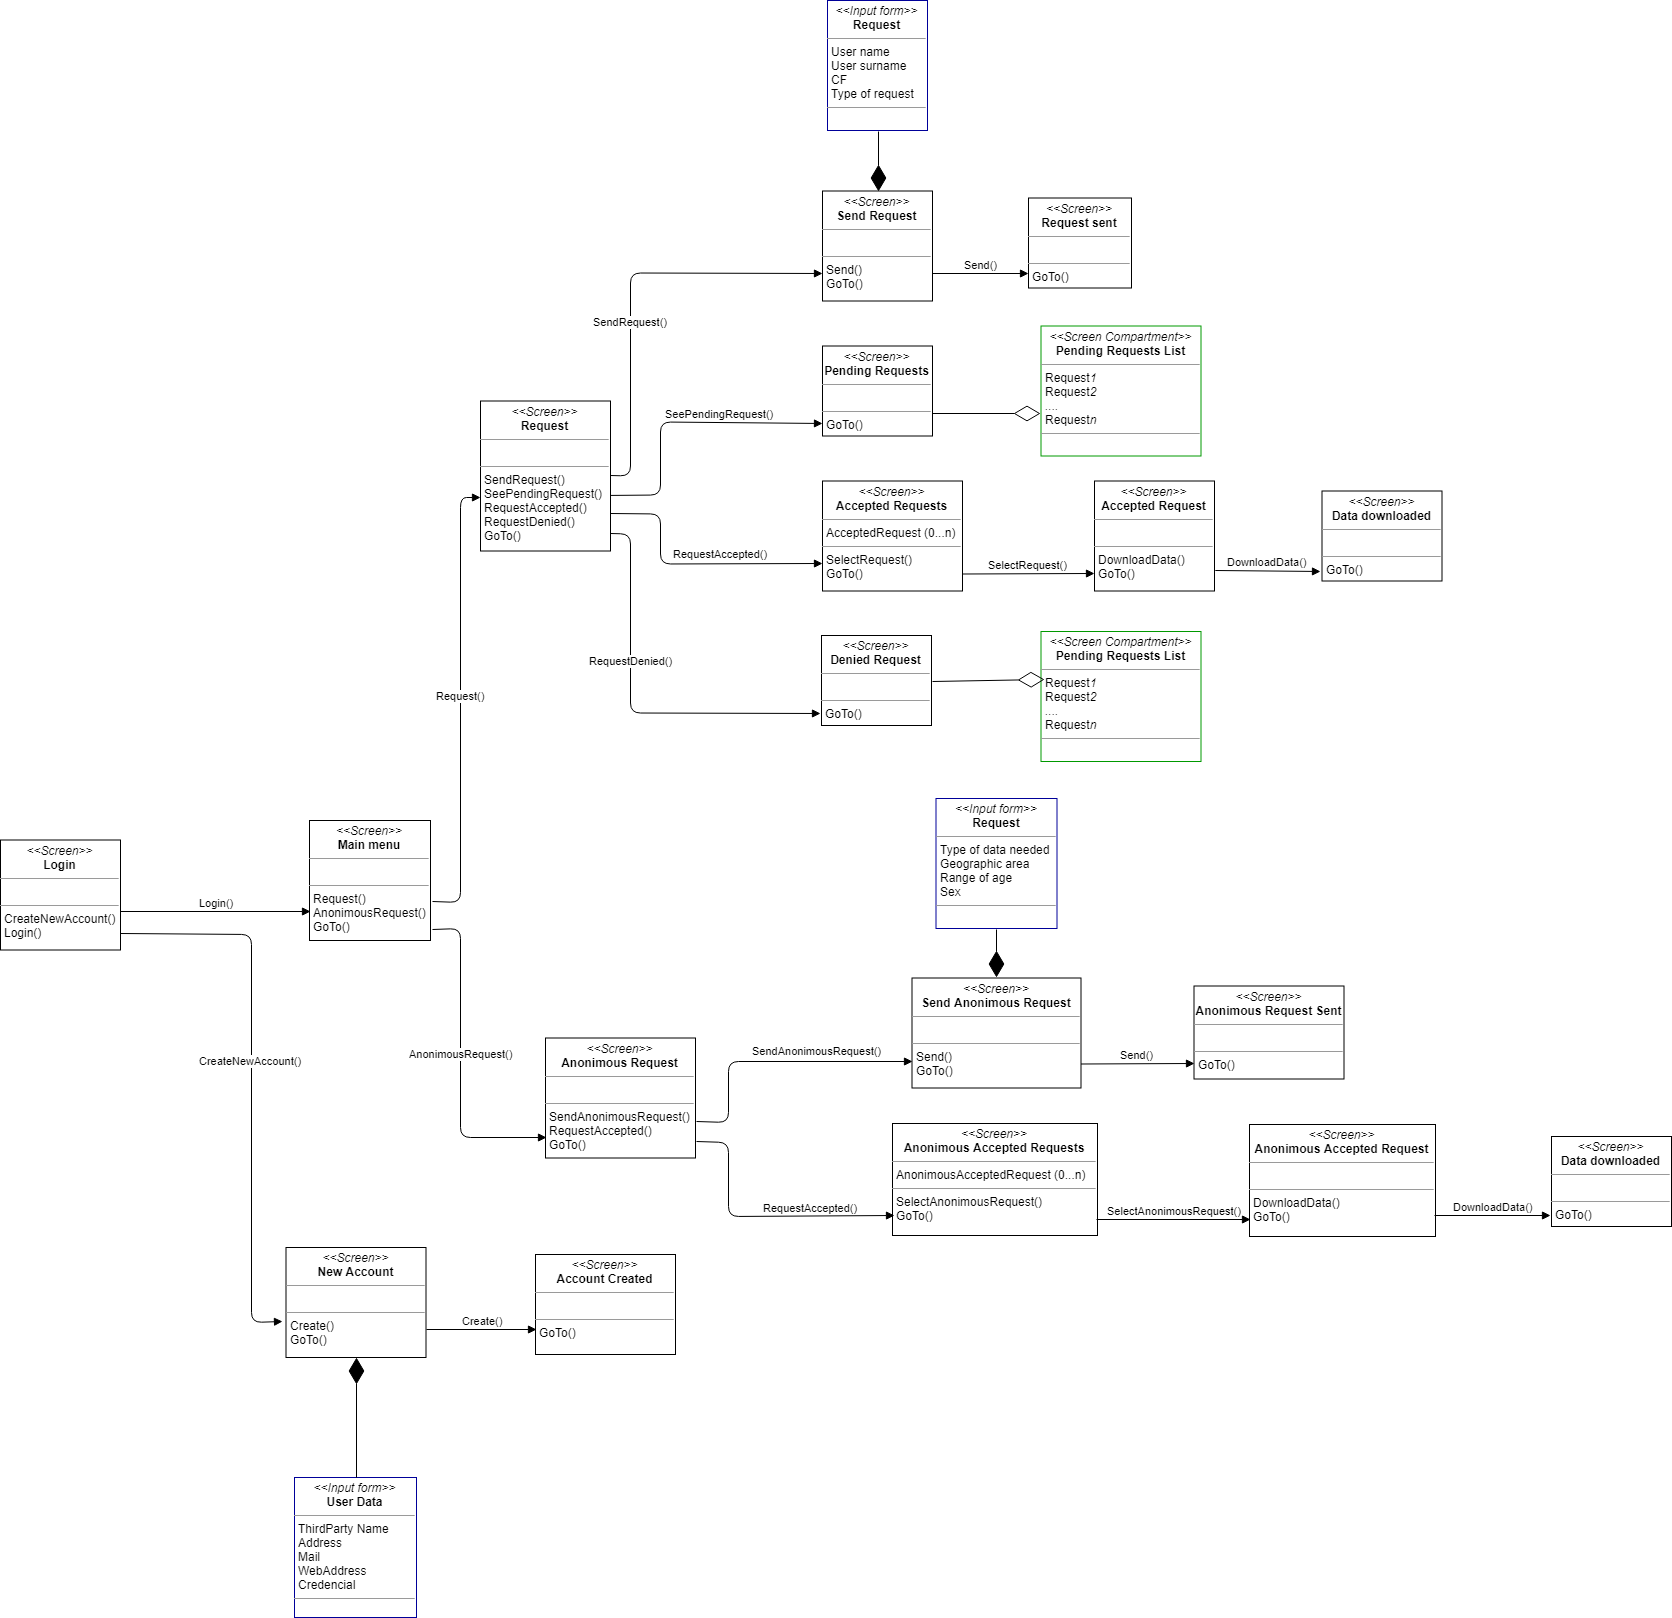
\includegraphics[scale=0.27]{Images/User_interface/Trackme-ThirdPartyD4H}
	\caption{Data4Help Third Party UX diagram}
\end{figure}

\newpage

{\color{Blue}{\subsubsection{AutomatedSOS}}}



\begin{figure}[H]
	\centering
	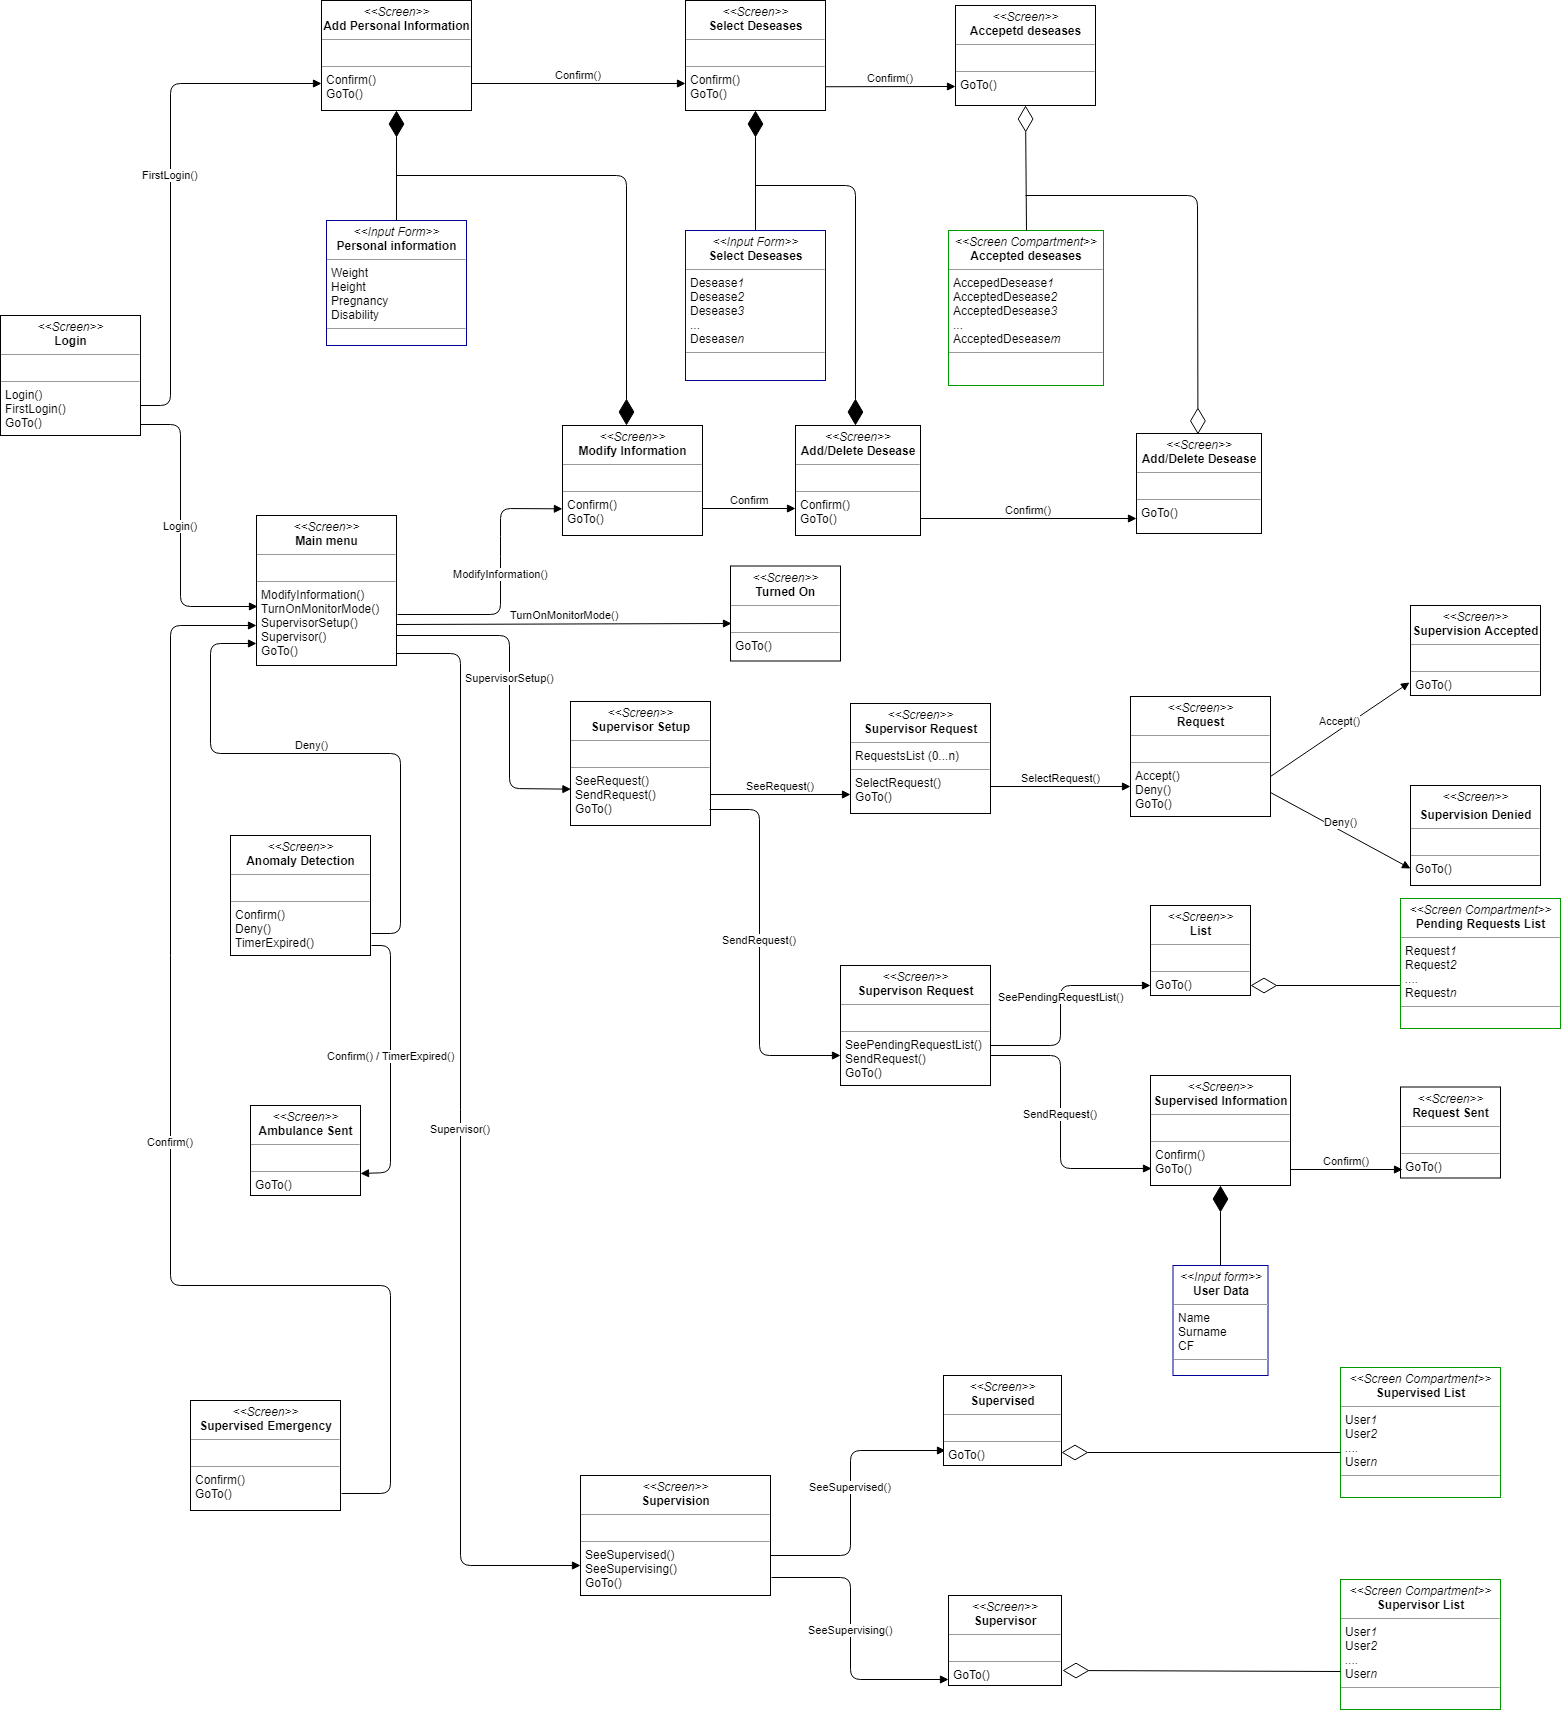
\includegraphics[scale=0.26]{Images/User_interface/Trackme-AutomatedSos}
	\caption{AutomatedSOS user UX diagram}
\end{figure}


\end{flushleft}